\section*{Testdesign}
%
Til undersøgelsen bruges robotten, der er illustreret på \autoref{fig:experiment}. Hver testperson bliver stillet overfor robotten fire gange, hvor robotten har hovedet indstillet i fire forskellige positioner. De fire positioner er illustreret på \autoref{fig:pos1}, \autoref{fig:pos2}, \autoref{fig:pos3} og \autoref{fig:pos4} og har følgende vinkler mellem vandret position:\blankline
%
Position 1: 100 $^{\circ}$\\
Position 2: 90 $^{\circ}$\\
Position 3: 45 $^{\circ}$\\
Position 4: 0 $^{\circ}$\blankline
%
For at balancere stimulipræsentationerne bruges et Latin Square design to gange, hvor testpersonerne bliver udsat for stimuli i følgende rækkefølgen beskrevet i \autoref{tab:Latin}.\blankline
%
\begin{table}[H]
	\centering
	\begin{tabular}{l|c}
		Tetsperson     & Præsentationsrækkefølge af position \\\hline
		Testperson 1   & 1 - 2 - 3 - 4          \\\hline
		Testperson 2   & 2 - 3 - 4 - 1          \\\hline
		Testperson 3   & 3 - 4 - 1 - 2          \\\hline
		Testperson 4   & 4 - 1 - 2 - 3          \\\hline
		Testperson 5   & 1 - 2 - 3 - 4          \\\hline
		Testperson 6   & 2 - 3 - 4 - 1          \\\hline
		Testperson 7   & 3 - 4 - 1 - 2          \\\hline
		Testperson 8   & 4 - 1 - 2 - 3   
	\end{tabular}
	\caption{Præsentationsrækkefølgen af robottens hovedposition.}
	\label{tab:Latin}         
\end{table}
\noindent
%
Testen udføres i kantinen på Fredrik Bajers vej 7, for at simulere et befolket område som eksempelvis en lufthavn. 


%What are your stimuli?

%
\begin{figure}[H]
\centering
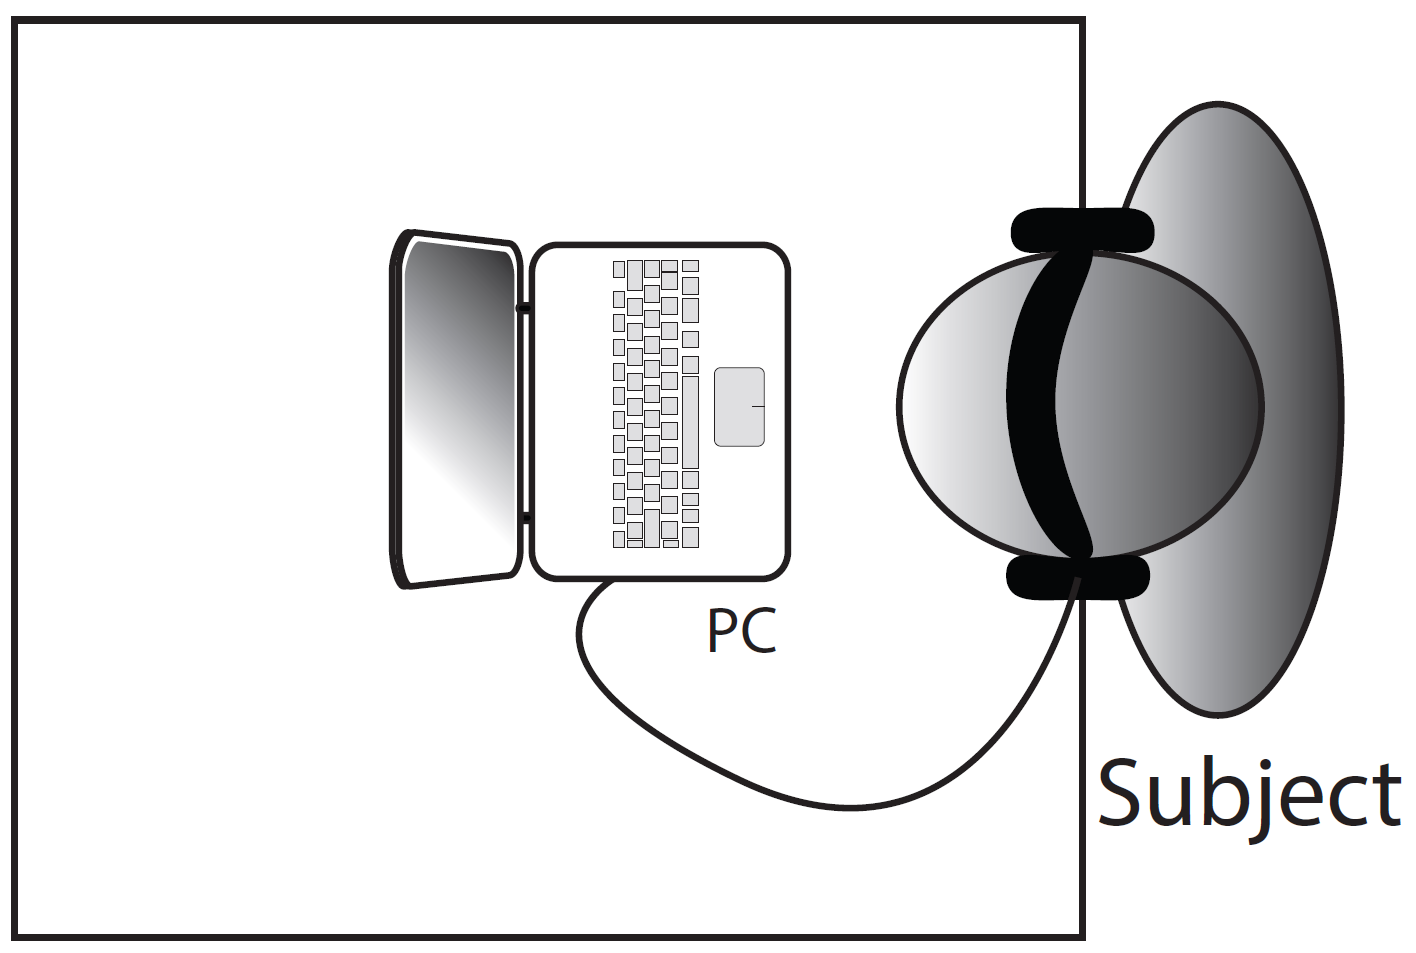
\includegraphics[width = 0.5\textwidth]{Figure/experiment.png} 
\caption{A sketch of the experimental setup.}
\label{fig:experiment}
\end{figure}
%
\subsection*{Scale design}
%Design the scale - argue for the choice and look of the scale.

\subsection*{Test subjects}
%Carry out the scaling experiment on a few subjects (preferably not yourself).
